It is assumed that programmer uses WSL 2 under Windows 10 in order to work with VM via the SSH\@.
By default, SSH keys are stored under the path \texttt{c/Users/username/.ssh}.
Assume that RSA key-pair is stored there and have the names \texttt{id\_rsa} and \texttt{id\_rsa.pub} for private
and public keys respectively.
In order to interact the VM via SSH it is necessary to copy RSA keypair to the WSL \texttt{username/.ssh} folder,
we use the commands under WSL
\begin{itemize}
    \item \texttt{cp /mnt/c/Users/pkolosov/.ssh/id\_rsa ~/.ssh/}
    \item \texttt{cp /mnt/c/Users/pkolosov/.ssh/id\_rsa.pub ~/.ssh/}
\end{itemize}
Then connection is available now using the command
\begin{itemize}
    \item \texttt{ssh -i ~/.ssh/id\_rsa razumovsky\_r@MachineStaticIP}
\end{itemize}
\begin{figure}[H]
    \centering
    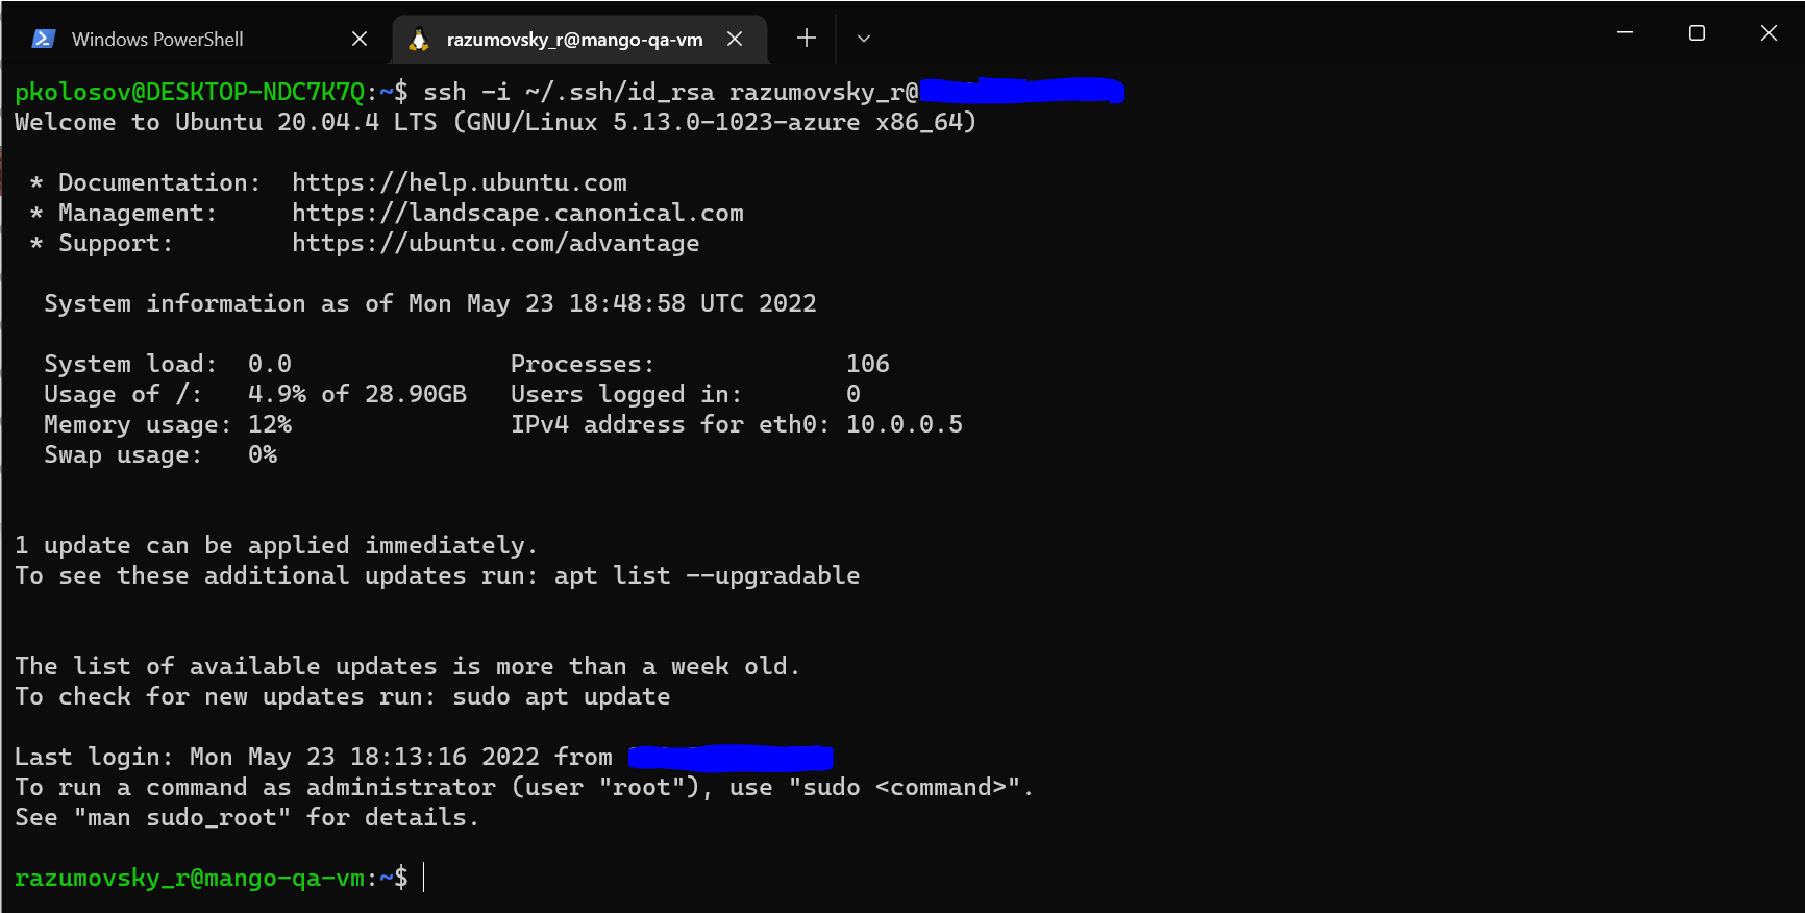
\includegraphics[width=1\textwidth]{img/01_ssh_connected}
    ~\caption{SSH connected successfully.}\label{fig:figure}
\end{figure}
